\documentclass[border=10pt]{standalone}

\usepackage{tikz}
\usepackage{tikzsymbols}
\usetikzlibrary{calc,patterns,shapes.geometric}

\def\centerarc[#1](#2)(#3:#4:#5){\draw[#1] ($(#2)+({#5*cos(#3)},{#5*sin(#3)})$) arc (#3:#4:#5);}

\begin{document}
	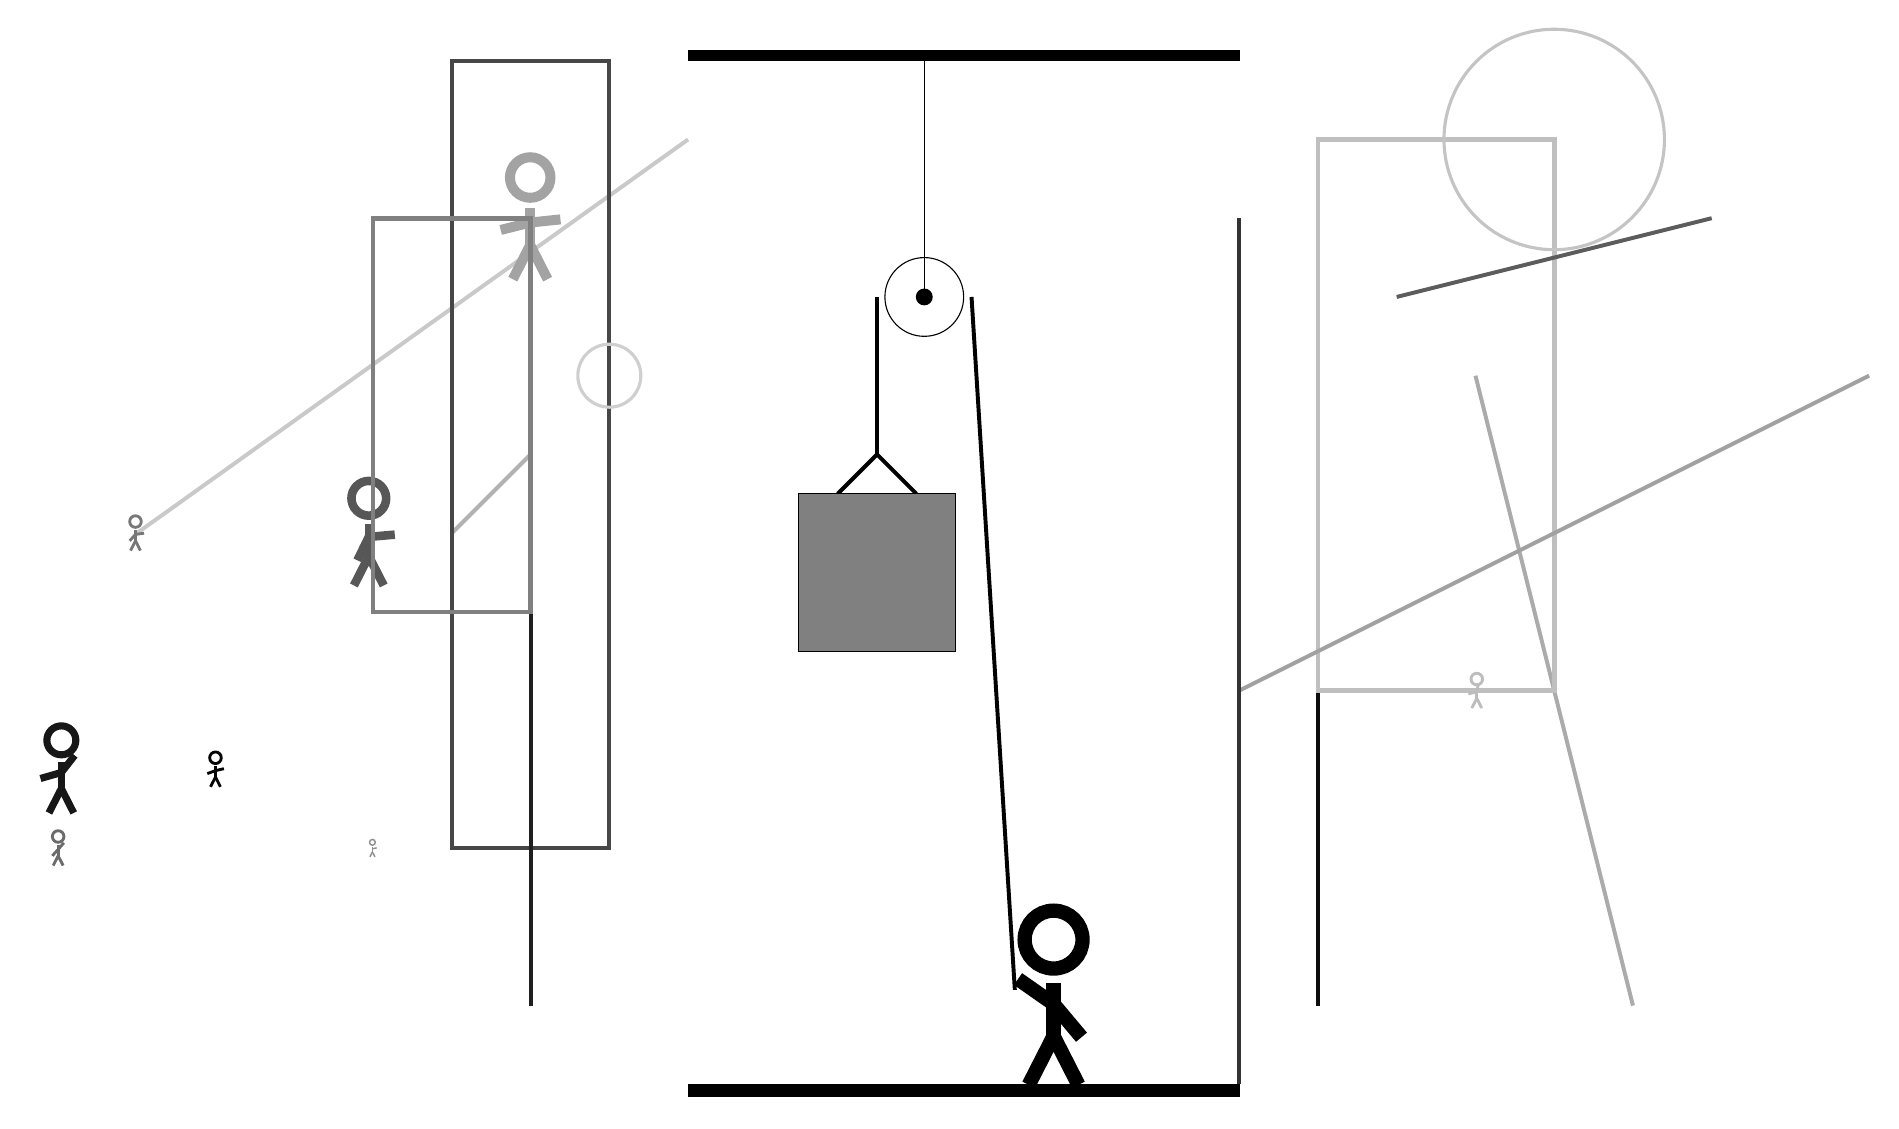
\begin{tikzpicture}
		%%%%% START %%%%%
		
		\draw[fill=black] (-2, 10) rectangle (5, 10.125);
		
		\draw (1, 7) circle (0.5);
		\draw[fill=black] (1, 7) circle (0.1);
		\draw (1, 10) -- (1, 7);
		
		\draw[line width=0.5mm, color=black!30](-4, 5) -- (-5, 4);
		
		\node[line width=0.5mm, color=black!58] at (-10, 0) {\Strichmaxerl[2][48][49]};
		\draw[line width=0.5mm, color=black!95](6, 6) -- (6, -2);
		\draw[line width=0.5mm, color=black!33](10, -2) -- (8, 6);
		\draw[line width=0.6mm, color=black!25] (6, 2) rectangle (9, 9);
		\draw[line width=0.5mm, color=black!76] (5, 4) rectangle (5, -1);
		
		\draw [line width=0.4mm, color=black!23](9, 9) circle (1.4);
		\node[line width=0.6mm, color=black!91] at (-10, 1) {\Strichmaxerl[5][16][52]};
		\draw[line width=0.5mm, color=black!64](7, 7) -- (11, 8);
		
		\draw[line width=0.5mm, color=black!21](-2, 9) -- (-9, 4);
		\node[line width=0.7mm, color=black!44] at (-6, 0) {\Strichmaxerl[1][90][12]};
		\node[line width=0.7mm, color=black!98] at (-8, 1) {\Strichmaxerl[2][20][13]};
		\draw[line width=0.5mm, color=black!72] (-3, 0) rectangle (-5, 10);
		\draw[line width=0.5mm, color=black!37](5, 2) -- (13, 6);
		\node[line width=0.2mm, color=black!53] at (-9, 4) {\Strichmaxerl[2][48][8]};
		\node[line width=0.4mm, color=black!66] at (-6, 4) {\Strichmaxerl[6][64][5]};
		
		\node[line width=0.6mm, color=black!36] at (-4, 8) {\Strichmaxerl[7][14][6]};
		\draw[line width=0.5mm, color=black!80](5, -3) -- (5, 8);
		\draw[line width=0.5mm, color=black!88](-4, -2) -- (-4, 8);
		\draw [line width=0.4mm, color=black!19](-3, 6) circle (0.4);
		\node[line width=0.7mm, color=black!26] at (8, 2) {\Strichmaxerl[2][13][79]};
		
		\draw[line width=0.6mm, color=black!50] (-4, 3) rectangle (-6, 8);
		
		
		\draw[line width=0.5mm] (-0.1, 4.5) -- (0.4, 5.0) -- (0.9, 4.5);
		\draw[fill=black!50] (-0.6, 4.5) rectangle (1.4, 2.5);
		
		\draw[line width=0.5mm] (0.4, 7) -- (0.4, 5.0);
		\centerarc[line width=0.5mm](1, 7)(0:180:0.6);
		\draw[line width=0.5mm](1.6, 7) -- (2.15, -1.8);
		
		\node at (2.6, -1.9) {\Strichmaxerl[10][-35][-50]};
		
		\draw[fill=black] (-2, -3) rectangle (5, -3.15);
		
		%%%%% END %%%%%
	\end{tikzpicture}
\end{document}